

\begin{frame}{Machine Learning Methods}
    \begin{center}
        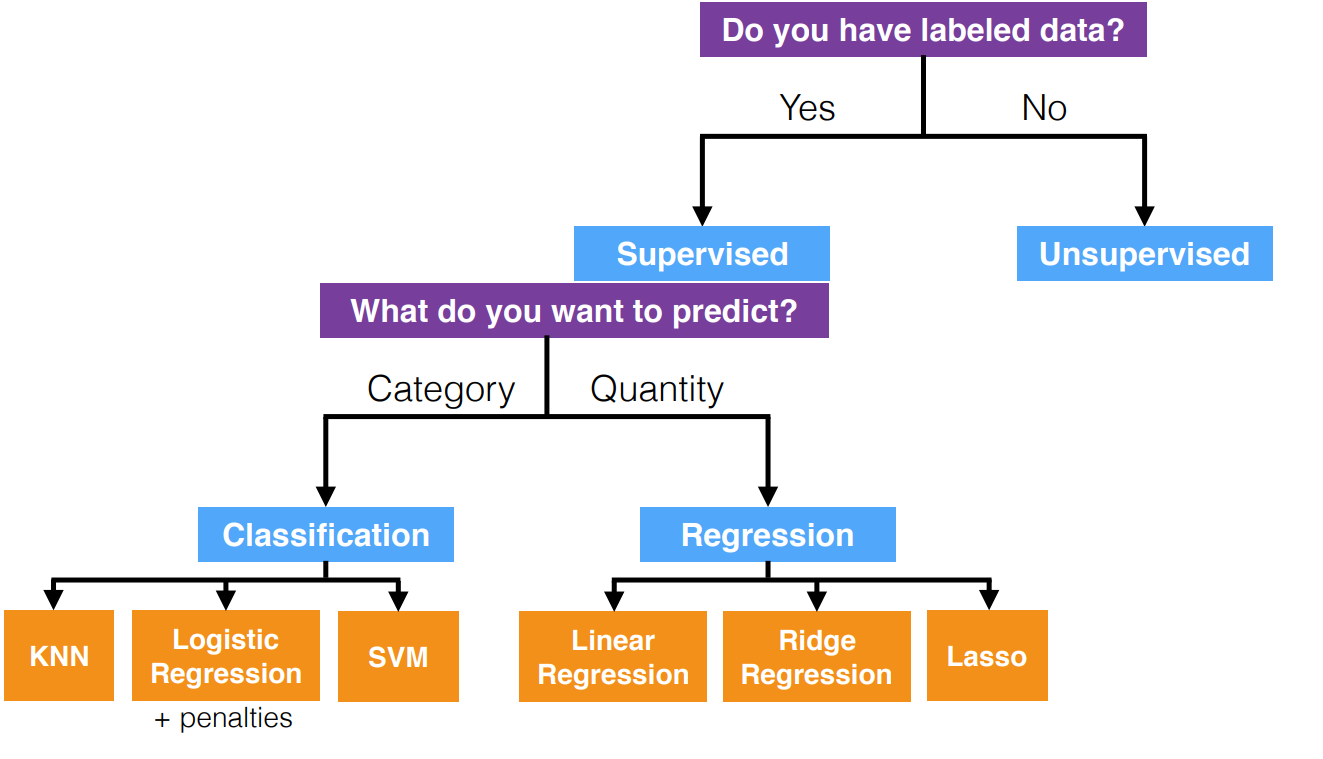
\includegraphics[width=0.95\linewidth]{images/support-vector-machines/support-vector-machines-1.png}
    \end{center}
\end{frame}


\begin{frame}{Support Vector Machines}
Support vector machine (SVM) is a supervised method for binary classification (two class). It is a generalization of 1 and 2 below.

\begin{enumerate}
    \item \textbf{Maximal margin classifier:} only applicable to linearly separable data.
    \item \textbf{Support vector classifier:} can be applied to data that is not linearly separable. Decision boundary still linear.
    \item \textbf{Support vector machine:} non-linear decision boundary.
\end{enumerate}
\end{frame}
